\chapter{Discussion}
\label{c:discussion}

Complementing the results of the previous chapter, a discussion follows, with negative and positive remarks about the general outcome of the thesis. \sref{s:discussion:limitations} presents the identified limitations of the study. On the other hand, the strengths and drawbacks of the methodological framework (or research design) are analysed in \sref{s:discussion:methodological-results}.

\section{Limitations of the research}
\label{s:discussion:limitations}
Regarding the methods used throughout the thesis, a series of pitfalls have been identified. First and foremost, the development of the SSP1-MOB qualitative narrative, as well as the subsequent backcasting process, could and probably should have been performed on the basis of a participatory process. Even though the normative approach of those sections has a higher saliency for policy and decision makers, the legitimacy of the results might have been compromised, because ``divergent values''\footnote{The thesis' results promote changes in cultural, technological and societal values in order to achieve a transition.} are incorporated without consultation with stakeholders or any other ``democratic'' approach \parencite{rounsevell2010_Developingqualitativescenario}. However, the scientific credibility of the thesis is well supported by the literature used and, in the particular case of the SSP1-MOB narrative, by being backed by the highly acknowledged scenario framework of the IPCC.

With respect to the AUTOLOCK conceptual model, it is clear that the CLDs developed are not the ultimate depiction of the automobility system. They are not even the \emph{only} possible representation of the aspects they are modelling---again, a participatory approach to their development, such as Group Model Building, would incorporate more points of view, eliciting the most important variables and links in the system \parencite{laurenti2014_GroupModelBuilding}. Rather, the AUTOLOCK model should be seen as an example of the potential that CLDs have for (a) describing system feedback structures and (b) conveying that information in an understandable way for decision makers and (transition) researchers alike. Many other perspectives could have been taken to model the automobility system, at this highly abstract level. The approach taken in this thesis for each of the AUTOLOCK model components is meant to provide enough basis for a discussion of the dynamic behaviour of the automobility system. Furthermore, the focus on abstract concepts and the loose system boundary (e.g., the inclusion of ideological discourses in the culture legitimation perspective) try to illustrate the difficulty in dealing with such a complex issue.

Another limit of the thesis lies in the breadth of the system perspective used. It is very complex and burdensome to include all the relevant aspects in a discussion of sustainable futures. For example, the fuel/energy discourse that permeates many transport studies is not explored in-depth in this thesis, nor is the technological dimension, in more general terms (new vehicle technologies, efficiency improvements, etc.). However, the constrained time and resources available to conduct this research do not allow for a further expansion of the system boundaries. Anyhow, it was a deliberate decision to shift the focus of this study onto the socio-cultural dimensions of the mobility system, following the hypothesis formulated in the \nameref{s:intro:aim-objectives} section.

Finally, the lack of (extensive) quantitative figures in either of the methodological perspectives used throughout the thesis (the backcasting process, the CLD model, etc.) poses a potential limitation to the credibility of the results. Scientific (natural sciences), engineering, economics and planning/policy research communities are used to quantitative evaluations and trust the scientific accuracy of studies when formal modelling has been performed. However, the socio-cultural focus of the thesis and the use of narratives, backcasts and transition perspectives actually brings it closer to social sciences. Furthermore, it is the opinion of the author that providing figures in a normative description of mobility futures, without the use of participatory methods, would render the results as non-credible and liable to huge biases.

\section{Methodological results}
\label{s:discussion:methodological-results}
Despite some limitations, there are some strong positive outcomes from this study. The methodological framework designed for the thesis manages to combine two seemingly dis-aligned approaches to futures studies: forecasting (in the form of CLDs) and backcasting. While there are articles in the literature of similar efforts, such as \textcite{kok2011_Combiningparticipativebackcasting} and \textcite{dortmans2005_Forecastingbackcastingmigration}, the difference lies in the integration method used in this research: the Multi-Level Perspective on sustainable transitions. \fref{f:discussion-methodology} presents a conceptual visualisation of the integration role that transitions theory plays in the thesis. To understand the importance of the contribution of this study, the following paragraphs describe the drawbacks of adhering to a single approach for policy assessment (either forecasting or backcasting). It is argued that the use of the MLP overcomes those limitations, thus becoming a prominent ``result'' of this thesis.

\begin{figure}
\centering
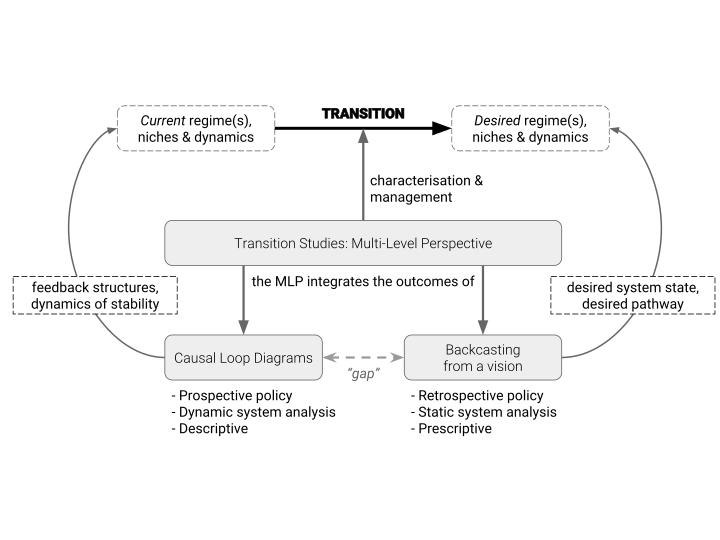
\includegraphics[clip,trim=0 3cm 0 3cm,width=\linewidth]{figures/discussion-methods.pdf}
\caption[Integrative power of transition theory]{Transition theory can bridge the gap between futures studies and forecasting tools, by translating the insights from each into the same language (discourse).}
\label{f:discussion-methodology}
\end{figure}

On one hand, forecasting tools (CLDs and System Dynamics, for example) are commonly used to inform policy makers of the possible development scenarios, but fail to convey normative insights: they are inherently \emph{descriptive} methods. Another weakness of using forecasts as the basis for policy making is that no space is available for radical innovation. This is, predictions based on present system structures cannot take into account structural change or unexpected developments. The policies that emerge from using forecasts are \emph{prospective}. On the other hand, the strength of forecasts and System Dynamics (CLDs) in particular, is the capability to analyse \emph{dynamic}\footnote{Again, the dynamism captured by these tools is constrained to the modelled structure of the system.} behaviours. Dynamics and feedback structures are very important to policy assessment, because they are sources of policy resistance mechanisms, such as rebound effects.

Backcasting and ``desirable'' visions methods are, on the contrary, normative in nature, this is, they are \emph{prescriptive} in their analysis (or discussion) of the systems under scope. However, unless explicitly incorporated in the processes, the perspective of the systems is rather \emph{static}. Even though they are used to convey the desired changes (dynamism over time), they do not account for feedback structures nor for dynamic system behaviour. In the context of sustainable transitions, a final feature of backcasting is appealing as a methodology: the \emph{retrospective} approach to policy design. The fact that backcasting processes start from a desired end-state opens the possibility to include radical innovation or, simply, ``radical'' changes that would be unthinkable from the present system condition.

The use of the MLP in the thesis as a discursive translation tool serves the purpose of overcoming the limitations described above, while benefiting from the strengths of each tool. (1) The focus on co-evolution and dynamism (stability and change) of socio-technical niches, regimes and landscapes fits perfectly the notion of system dynamics captured by CLDs. (2) While not normative per se, the MLP can still accommodate the results of a backcasted pathway to a normative future vision. (3) The context of a ``transition'' embeds desired future visions and pathways and, therefore, policy design can be made retrospectively, allowing broader possibilities to be included and for policies that support radical innovation. Finally, the multidisciplinary approach of the MLP supports an analysis scope broader than that of the formal models of System Dynamics, similarly to backcasting.

As the concluding remark, the aforementioned use of the MLP approach is, as argued, a significant contribution to sustainability research. It could, to some extent, be regarded as a form of \emph{transition management} \parencite{rotmans2001_Moreevolutionthan,kemp2011_TransitionManagementas}, although it differs in some aspects: different emphasis on culture, inclusion of subaltern combined methodologies and, following the transitions governance scheme described by \textcite{kemp2007_Transitionmanagementas}, this thesis is situated only at a strategic management level. However, the approach taken can benefit other sustainability studies in the following situations:
\begin{enumeratealpha}
\item A (participatory) process has delivered a desirable vision and/or pathway to a sustainable future, but there are uncertainties with regards to required structural changes or policy resistance mechanisms.
\item A forecasting study has provided decision makers with a thorough understanding of the current system and its feedback mechanisms but, even at the light of possible scenarios described by the forecast, they are unsure of what normative actions should be taken.
\end{enumeratealpha}
In both cases, a complementary study can be performed and the results can be then harmonised using an MLP approach. This integration framework is, indeed, the most interesting outcome of the thesis.

\section{Further research}
\label{s:discussion:further}
The main line of research that stems from the work in this thesis is the investigation of policy analysis frameworks. This is, researching whether transition theory, and the MLP in particular, can help in the design of policies that fit sustainability better than the current paradigm. In this respect, the scholars from the transitions management field have already made progress, but their approach is a little different. Whereas they focus on niche support and long term goals, this thesis also emphasises the ability of the MLP as an integrative narrative for more ``specific'' assessment tools.

A straightforward extension of the thesis would be to carry out the backcasting process (and the development of the qualitative narrative that serves as the guideline) in a participatory setting. This way, different policy results might be derived or, at the very least, confirmed and validated by stakeholders and general participants. Democracy is, unfortunately, a forgone aspect of sustainability studies. In the case of the thesis, due to time and resources constraints, but in a more general case, due to technocratic views on what science and research is all about. Lengthier study settings, such as PhD research or government officials could undertake this effort.

The usage of Causal Loop Diagrams in combination with other policy design mechanisms is an interesting contribution that deserves further work as well. Most of the literature on System Dynamics and CLDs deals with narrower scopes and bounded systems than what has been studied here. In particular, they are (almost) never used to model ``soft'' issue such as cultural frameworks. Despite the difficulty to quantify these aspects, the argument of this thesis is that CLDs could be used to mentally model these very important issues. They definitely serve the purpose of making mental models explicit, especially when developed in workshops or through Group Model Building techniques.

%The results are contrasted with the literature in \sref{s:discussion:coherency} and, finally,
%\section{Coherency with the literature}
%\label{s:discussion:coherency}
%The thesis is, despite the aforementioned limitations, aligned with the current body of literature on sustainable mobility futures. For example, \textcite{banister2008_sustainablemobilityparadigm} describes four main categories of action that must be pursued to reach the sustainable mobility paradigm he argues for:
\begin{enumerate}
\item Reduce the need for travel through substitution.
\item Encourage modal shift through transport policy measures.
\item Reduce trip lengths through sustainable spatial planning.
\item Encourage higher efficiency in transport through vehicle and fuel technology innovation.
\end{enumerate}
This thesis, on the other side, advocates for very similar results. The backcasted changes are also categorised in four main fronts of action: (1) cultural changes to reduce the overall mobility demand, (2) land-use changes to reduce trip lengths and demand, (3) encouraging modal shift through demand management and intermodal travel and (4) increase vehicle and fuel efficiencies. This similarity is no coincidence. Both \textcite{banister2008_sustainablemobilityparadigm} and this thesis are built on the realisation that the current and historic paradigm of mobility is obsolete from a sustainability point of view and both studies focus on the transformation (or transition) of the system into a new paradigm.



\todoparagraph{In general, the thesis ``outcomes'' are ``biased'', personal and not too generalizable. But! The combination of policy-making tools through the ``discoursive''/``narrative'' power of transition studies is a really interesting result. Even though more work needs to be devoted to this, it clearly suggests that by using the terminology of transition theories, we can bridge the gap between seeminlgy different approaches and tools. This can be very useful in the context of policy-making and (future(s)) sustainability studies, since it promises to deliver a more coherent and integrated result than other approaches.}